\chapter{Declaration}
\vspace*{2\baselineskip}
I declare that this thesis has been composed 
solely by myself and that it has not been submitted, either in whole or
in part, in any previous application for a degree.
Except where otherwise acknowledged, the work presented is entirely my
own.
\vspace{6\baselineskip}\\
\begin{flushright}
\hspace*{\fill}
Luiz Max Fagundes de Carvalho
\newline
4th December 2018

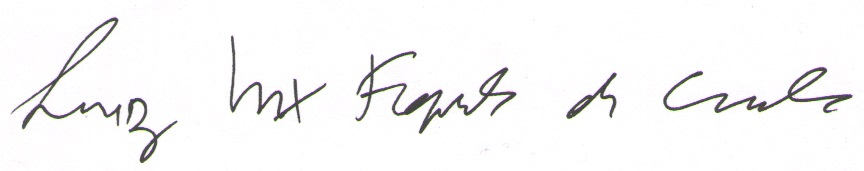
\includegraphics[scale=.35]{\dir/lmfcarvalho_sign}

\end{flushright}

\cleardoublepage

In Chapter 2, the idea to show that the mapping from phylogenies to inter-coalescent intervals and numbers of lineages is surjective non-injective was suggested to me by Professor Marc Suchard (UCLA).

Chapter 4 has been published as part of Dudas, G., Carvalho, L. M., Bedford, T. et al.(2017)~\textit{Nature}, 544(7650):309--315.

Chapter 5 has been published as part of Diehl, W., Lin, A.E., Grubaugh, N.D., Carvalho, L.M. et al. (2016)~\textit{Cell}, 167(4):1088--1098.

During the PhD I was a co-author in Rambaut, A., Lam, T. T., Carvalho, L. M.,  Pybus, O. G. (2016)~\textit{Virus Evolution} 2: vew007 and Dudas, G., Carvalho, L. M., Rambaut, A.,  Bedford, T. (2018)~\textit{ELife}, 7, e31257, which are not covered in this thesis.
